%%%%%%%%%%%%  Generated using docx2latex.com  %%%%%%%%%%%%%%

%%%%%%%%%%%%  v2.0.0-beta  %%%%%%%%%%%%%%

\documentclass[12pt]{report}
\usepackage{amsmath}
\usepackage{latexsym}
\usepackage{amsfonts}
\usepackage[normalem]{ulem}
\usepackage{soul}
\usepackage{array}
\usepackage{amssymb}
\usepackage{extarrows}
\usepackage{graphicx}
\usepackage[backend=biber,
style=numeric,
sorting=none,
isbn=false,
doi=false,
url=false,
]{biblatex}\addbibresource{bibliography.bib}

\usepackage{subfig}
\usepackage{wrapfig}
\usepackage{wasysym}
\usepackage{enumitem}
\usepackage{adjustbox}
\usepackage{ragged2e}
\usepackage[svgnames,table]{xcolor}
\usepackage{tikz}
\usepackage{longtable}
\usepackage{changepage}
\usepackage{setspace}
\usepackage{hhline}
\usepackage{multicol}
\usepackage{tabto}
\usepackage{float}
\usepackage{multirow}
\usepackage{makecell}
\usepackage{fancyhdr}
\usepackage[toc,page]{appendix}
\usepackage[hidelinks]{hyperref}
\usetikzlibrary{shapes.symbols,shapes.geometric,shadows,arrows.meta}
\tikzset{>={Latex[width=1.5mm,length=2mm]}}
\usepackage{flowchart}\usepackage[paperheight=11.69in,paperwidth=8.27in,left=1.0in,right=1.0in,top=1.0in,bottom=1.0in,headheight=1in]{geometry}
\usepackage[utf8]{inputenc}
\usepackage[T1]{fontenc}
\TabPositions{0.5in,1.0in,1.5in,2.0in,2.5in,3.0in,3.5in,4.0in,4.5in,5.0in,5.5in,6.0in,}

\urlstyle{same}

\renewcommand{\_}{\kern-1.5pt\textunderscore\kern-1.5pt}

 %%%%%%%%%%%%  Set Depths for Sections  %%%%%%%%%%%%%%

% 1) Section
% 1.1) SubSection
% 1.1.1) SubSubSection
% 1.1.1.1) Paragraph
% 1.1.1.1.1) Subparagraph


\setcounter{tocdepth}{3}
\setcounter{secnumdepth}{3}


 %%%%%%%%%%%%  Set Depths for Nested Lists created by \begin{enumerate}  %%%%%%%%%%%%%%


\setlistdepth{9}
\renewlist{enumerate}{enumerate}{9}
		\setlist[enumerate,1]{label=\arabic*)}
		\setlist[enumerate,2]{label=\alph*)}
		\setlist[enumerate,3]{label=(\roman*)}
		\setlist[enumerate,4]{label=(\arabic*)}
		\setlist[enumerate,5]{label=(\Alph*)}
		\setlist[enumerate,6]{label=(\Roman*)}
		\setlist[enumerate,7]{label=\arabic*}
		\setlist[enumerate,8]{label=\alph*}
		\setlist[enumerate,9]{label=\roman*}

\renewlist{itemize}{itemize}{9}
		\setlist[itemize]{label=$\cdot$}
		\setlist[itemize,1]{label=\textbullet}
		\setlist[itemize,2]{label=$\circ$}
		\setlist[itemize,3]{label=$\ast$}
		\setlist[itemize,4]{label=$\dagger$}
		\setlist[itemize,5]{label=$\triangleright$}
		\setlist[itemize,6]{label=$\bigstar$}
		\setlist[itemize,7]{label=$\blacklozenge$}
		\setlist[itemize,8]{label=$\prime$}

\setlength{\topsep}{0pt}\setlength{\parindent}{0pt}
\renewcommand{\arraystretch}{1.3}

\date{}


%%%%%%%%%%%%%%%%%%%% Document code starts here %%%%%%%%%%%%%%%%%%%%



\begin{document}

\begin{titlepage}
\sloppy
\begin{center}
BABE\c S BOLYAI UNIVERSITY, CLUJ NAPOCA, ROM\^ ANIA

FACULTY OF MATHEMATICS AND COMPUTER SCIENCE

\vspace{6cm}

\Huge \textbf{SMART DRIVING ASSISTANT}

\vspace{1cm}

\normalsize -- MIRPR report --

\end{center}


\vspace{5cm}

\begin{flushright}
\Large{\textbf{Team members}}\\
\begin{FlushRight}
{\fontsize{14pt}{16.8pt}\selectfont Marc Moldovan, Software Engineering, 258/2\par}
\end{FlushRight}\par

\begin{FlushRight}
{\fontsize{14pt}{16.8pt}\selectfont Tudor Maier, Software Engineering, 258/2\par}
\end{FlushRight}\par
\end{flushright}

\vspace{4cm}

\begin{center}
2020
\end{center}

\end{titlepage}
\par



\vspace{\baselineskip}

\vspace{\baselineskip}

\vspace{\baselineskip}

\vspace{\baselineskip}
\par

\vspace{\baselineskip}

\begin{abstract}
	This paper documents a research in which a new mobile application was developed for Android devices that will work as a smart co-pilot for the drivers. This product introduces real-time object detection for the phone camera on a various set of objects, together with location and weather service integration.
The idea of this application is to provide an easy-to-use mobile application with a user-friendly interface that will provide different information about the road.

\end{abstract}

 %%%%%%%%%%%%  This Produces Table Of Contents %%%%%%%%%%%%%%

\tableofcontents
\addcontentsline{toc}{chapter}{Table of contents}

\vspace{\baselineskip}

\vspace{\baselineskip}

\vspace{\baselineskip}

\vspace{\baselineskip}

\vspace{\baselineskip}

\vspace{\baselineskip}

\vspace{\baselineskip}

\vspace{\baselineskip}

\vspace{\baselineskip}

\vspace{\baselineskip}

\vspace{\baselineskip}

\vspace{\baselineskip}

\vspace{\baselineskip}

\vspace{\baselineskip}

\vspace{\baselineskip}

\vspace{\baselineskip}

\chapter{Introduction}
\section{What? Why? How?}
\begin{justify}
The auto industry has been growing lately, this automatically sporing the number of drivers. Having this in mind, the outcome has both advantages and disadvantages.
\end{justify}\par

\begin{justify}
The main disadvantages are pollution and the increase in the number of road accidents caused by careless driving as well as the failure to adjust the speed in different situations.\\
Currently, there are several ways to increase the driving experience, but these are either very expensive or require a high level of technical skills to use them.
\end{justify}\par

\begin{justify}
Also, the mobile app industry is growing insanely fast and there are more and more smart gadget users. Users prefer using mobile devices applications on behalf of other static devices such as personal computers or web applications because you have access to them at any time. 
\end{justify}\par

\tab Applying the reasons mentioned above, creating a mobile application with the purpose of road assistant can increase the safety of the drivers.\par

\tab In this paper, we want to present an easy-to-use application, which combines several concepts such as: machine learning, location services and third party services.\par

The application will be able to detect different objects and traffic participants such as: pedestrian crossings, traffic signs, pedestrians; but it will also calculate the speed at which the vehicle is moving and will warn you about adapting the speed to the present weather conditions.\par


\vspace{\baselineskip}
\section{Paper structure and original contribution(s)}
\begin{justify}
The research presented in this paper advances the theory, design, and implementation of several particular models.
\end{justify}\par

\begin{justify}
The main contribution of this report is to present a smart algorithm to solve the problem of detecting different objects in traffic as well as traffic participants. 
\end{justify}\par

\begin{justify}
The second contribution of this report consists of building an intuitive, easy-to-use and friendly mobile application. Our aim is to build an assistant that will help drivers identify objects in traffic faster. Based on the results of the algorithm, it is possible to display on the screen the possible dangers as well as what they should be aware of at that time.
\end{justify}\par

\begin{justify}
The third contribution of the paper is the integration of a third party application that provides weather data with a location service so that the driver can be notified when he has to reduce the speed to adapt to the weather conditions at that time. Moreover, it is desired to notify the driver when it exceeds the speed limit.
\end{justify}\par

\begin{justify}
The present work contains 10 bibliographical references and is structured in five chapters as follows:
\end{justify}\par

\begin{justify}
The first chapter is a short introduction in the paper where the reasons behind it are presented and how it is structured.
\end{justify}\par

\begin{justify}
The second section describes the scientific problem behind the paper and what are the advantages and disadvantages of using machine learning.
\end{justify}\par

\begin{justify}
The third chapter presents the theories and applications used so far to solve the problem of the work.
\end{justify}\par

\begin{justify}
The fourth section describes the approach for solving the stated problem.
\end{justify}\par

\begin{justify}
The fifth chapter presents the developed application and its results.
\end{justify}\par

\begin{justify}
The sixth section describes the conclusions and future work.
\end{justify}\par

\tab 
\vspace{\baselineskip}
\vspace{\baselineskip}
\chapter{Scientific problem}
\begin{justify}
Automobiles capable of transporting human people have already been invented for over 100 years ago, therefore, now, people have already gotten accustomed to driving and tend to get distracted due to other external factors, such as other people in the car, phone ringing, listening to music and so on. 
\end{justify}\par

\begin{justify}
Taking into account this matter, the drivers’ and pedestrians’ safety is at risk and requires another approach, other than the usual laws, which the drivers/pedestrians tend to break them more and more. 
\end{justify}\par

\begin{justify}
Ultimately, having access to easy-to-use Artificial Intelligence tools $\&$  algorithms can lead to the development of autonomous cars or system that will prevent the dangers on the road and reduce the risk in traffic.
\end{justify}\par

\chapter{State of the art}
The need of a smart artificial co-pilot was already noticed by the car manufacturers and all of them started to invest into this direction in the past few years. Each of them tries to find an optimal solution, but it involves different additional costs, for example: attaching new sensors and cameras to the car, collecting data and displaying them in a human-friendly form, attaching a graphical interface on the main console of the car to extend the infotainment system. \par

BMW has one of the Intelligent Driving Assistant on the market. It offers different features such as camera-based system for detecting vehicles around the car, Person warning for pedestrian detection and notifying the driver of possible dangers. Moreover, they also offer speed limit information depending on the location of the vehicle and recommend new speed limits depending on the weather conditions. In addition, they include many useful features: BMW Night Vision, head-up display, parking assistant and surround view of the car [10].\par


\vspace{\baselineskip}

\vspace{\baselineskip}


%%%%%%%%%%%%%%%%%%%% Figure/Image No: 1 starts here %%%%%%%%%%%%%%%%%%%%

\begin{figure}[H]
\advance\leftskip 0.02in		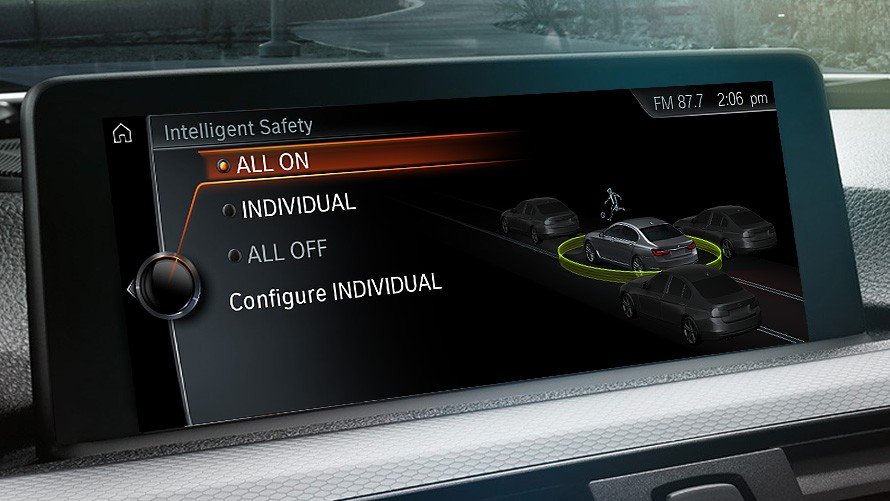
\includegraphics[width=5.06in,height=2.85in]{./media/image10.png}
\end{figure}


%%%%%%%%%%%%%%%%%%%% Figure/Image No: 1 Ends here %%%%%%%%%%%%%%%%%%%%

\par

Fig. 3.1. Lane keeping assistant from BMW [10]\par


\vspace{\baselineskip}

\vspace{\baselineskip}

\vspace{\baselineskip}

\vspace{\baselineskip}
\chapter{Proposed approach}
\begin{justify}
Driving assistant has been implemented on an Android platform, being one of the most used devices and also offering different useful sensors, such as gps location and camera recording. Moreover, we can make use of the size of this Android device to make it mobile and easy to use and mounted on a vehicle. The Android application aims to detect the different traffic signs (pedestrian crossing sign, traffic light), road markings (pedestrian crossing), as well as pedestrians on the sidewalk or pedestrian crossing.
\end{justify}\par

\begin{justify}
In order to detect certain signs, objects, markings or traffic participants, an Object detection algorithm is required. So this was our main challenge.
\end{justify}\par

\begin{adjustwidth}{0.5in}{0.0in}
\section{TensorFlow Object Detection API with SSD model}
\end{adjustwidth}

\begin{justify}
\tab TensorFlow\ Object Detection API is $``$an open source framework built on top of TensorFlow$"$  that aims to make it easy to $``$construct, train and deploy object detection models$"$  [1].  Along with the API they provide a few pre-trained models such as ssd\_mobilenetv2 and faster r-cnn2. 
\end{justify}\par

\tab MobilenetV2\  is neural network architecture published by Google that was optimized for mobile devices. Mobilenet is a pre-trained model which was trained using COCO Dataset (Common Objects in Context) which consists of over 300 thousand images and over 200 thousand labeled classes. It contains 91 object types such as $``$person$"$ , $``$traffic light$"$ , $``$car$"$  [2]. \\
\tab With\ the new version of the Mobilenet model, Google provided a new architecture which contains two types of blocks: residual and for downsizing. Also, there are three layers for both types of blocks [3].  Residual blocks connect the beginning and end of a convolutional block with a skip connection. By adding these two states the network has the opportunity of accessing earlier activations that weren’t modified in the convolutional block. This approach turned out to be essential in order to build networks of great depth. MobileNetV2 follows a narrow->wide->narrow approach. The first step widens the network using a 1x1 convolution because the following 3x3 depthwise convolution already greatly reduces the number of parameters. Afterwards another 1x1 convolution squeezes the network in order to match the initial number of channels [4].\par

\tab \tab \tab \tab 
\vspace{\baselineskip}

%%%%%%%%%%%%%%%%%%%% Figure/Image No: 2 starts here %%%%%%%%%%%%%%%%%%%%

\begin{figure}[H]
\advance\leftskip 0.0in		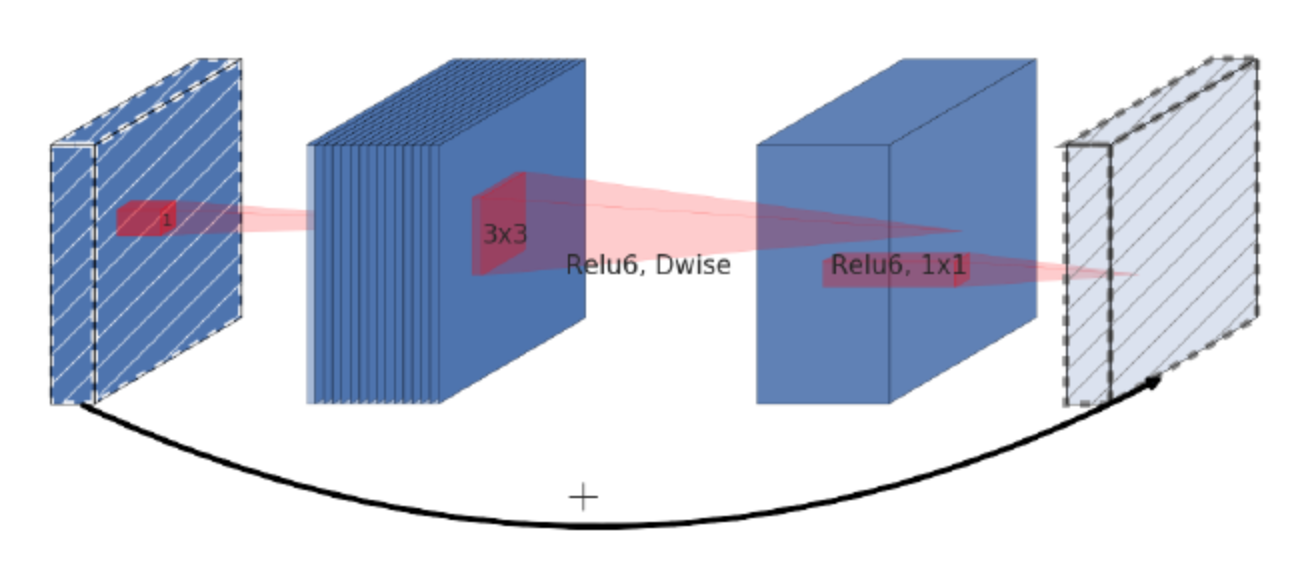
\includegraphics[width=6.27in,height=2.72in]{./media/image4.png}
\end{figure}


%%%%%%%%%%%%%%%%%%%% Figure/Image No: 2 Ends here %%%%%%%%%%%%%%%%%%%%

\begin{adjustwidth}{1.5in}{0.0in}
Fig. 4.1 Residual block [4]\par

\end{adjustwidth}


\vspace{\baselineskip}

\vspace{\baselineskip}

\vspace{\baselineskip}

\vspace{\baselineskip}
\begin{justify}
Faster R-CNN is one of the most famous detection architecture that uses convolution neural networks like YOLO (You Only Look Once) or SSD (Single Shot Detector) [5]. This model is trained independently with weights from a network trained for an ImageNet classification task. ImageNet is an image database with over 14 millions images and 21841 synset indexed with classes like $``$person$"$  [6]. Faster R-CNN is composed of three parts.
\end{justify}\par



%%%%%%%%%%%%%%%%%%%% Figure/Image No: 3 starts here %%%%%%%%%%%%%%%%%%%%

\begin{figure}[H]
	\begin{Center}
		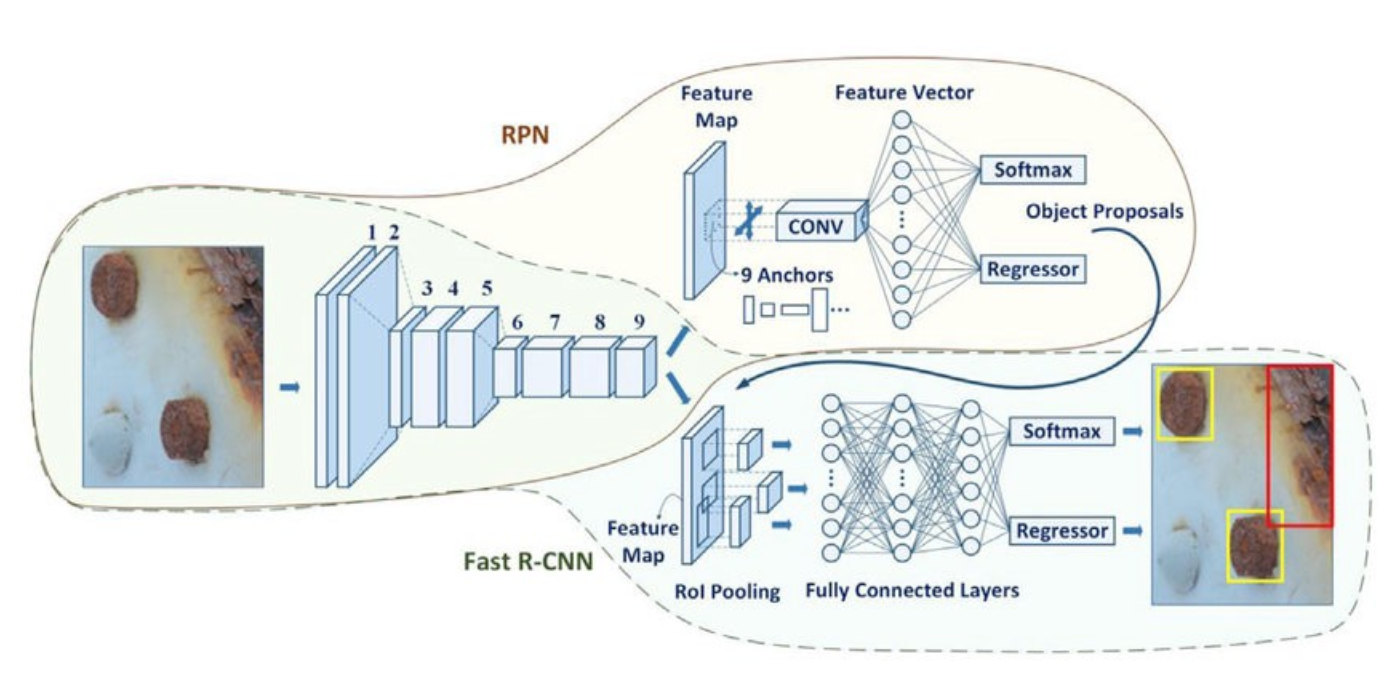
\includegraphics[width=6.27in,height=3.08in]{./media/image6.png}
	\end{Center}
\end{figure}


%%%%%%%%%%%%%%%%%%%% Figure/Image No: 3 Ends here %%%%%%%%%%%%%%%%%%%%

\par

\begin{justify}
\tab \tab \tab Fig 4.2. Faster R-CNN architecture [5].
\end{justify}\par


\vspace{\baselineskip}

\vspace{\baselineskip}
First part is the convolutional layer. Here the filters are trained to extract features from image. These filters are filtering our input image and are extracting just a feature map of the image by eliminating pixels with low values [5].\\
\tab The second part is the Region Proposal Network (RPN) which is a small neural network sliding on the last feature map of the convolution layers and predict whether there is an object or not and also predict the bounding box of those objects [5].\par

The last part consists of Classes and Bounding Boxes is defined by taking the input from the RPN and predict object class (classification)\par

\section{Data formatting and collecting}
\begin{justify}
\tab The first thing that we had to do in order to train a custom model is to collect data. So we picked a set of images from google maps street view. After selecting different $``$driving situations$"$ . 
\end{justify}\par

\tab Secondly,\ to improve the learning speed we had we need to resize our images before annotating them.  at a resolution of 800 x 800. We have done this with the help of PhotoShop scripts. After the resize, we split the images into two directories: $``$train$"$  and $``$test$"$ . We picked a ration between these of 20$\%$  - 80$\%$ .\par

\tab Lastly, the annotation phase was done using an open LabelImg tool. This tool, will generate $``$xml$"$  files with the position of desired object. This tool saves the $``$xml$"$  files in a format supported by both ImageNet and SSD [7].\par

\section{Google location service}
\tab One of the most important features of the mobile devices is the location awareness. The location API is available through the Google Play Services and enabling it in the application will provide location tracking, geofencing and activity recognition. \\
\tab Using the location service we can determine the speed current speed. We can do this by storing the previous location and always compare it with the current one. We used the following formula:\par

 \( s = \sqrt{ \left( x_{1} - x_{2} \right) ^{2}+ \left( y_{1} -y_{2} \right) ^{2}^{}}~/   \left( t_{1} - t_{2} \right)  \) \par


\vspace{\baselineskip}
s - speed\par

x1, y1 - current longitude and latitude\par

x2, y2 - last longitude and latitude\par

t1, t2 - current time and last location registration time\par

\section{AccuWeather Api}
\begin{justify}
\tab AccuWeather is a company that provides weather forecasting services worldwide. It also has an open API that we can consume [9]. Combined with Google Location Services we will get our current location weather data. 
\end{justify}\par

\chapter{Application}
\section{Methodology}
In order to re-train a pre-trained model, images taken from Google Maps with Street View functionality were used in order to obtain real images and a slightly various dataset.\par

After gathering around 30 images, the next step was to process them in order to achieve better performance time for the training phase, therefore a batch resize was executed with Photoshop in order to reduce the size of the images to around 800px x 800px. \par

Furthermore, to train the object detection model, the images needed to be labeled in order to detect a specific set of classes. For this phase, an open-source tool was used, named LabelImg, which can be found on GitHub and is easy to use for labeling the objects within a dataset.\par

The labeled images were split into 2 groups, one for training phase and one for testing phase, the recommended ratio is said to be somewhere around 80$\%$  training images and 20$\%$  testing images. An important mention here, is the fact that the testing images must be different from the training images in order to receive correct results of the model’s efficiency.\par

\section{Data}
The data used was simply taken from Google Maps using the Street View functionality. The images were taken from various angles, zoom level and distance in order to efficiently train the model.\par

The images are real images taken from the real world, therefore the obtained model should be more accurate.\par

\section{Results}


%%%%%%%%%%%%%%%%%%%% Figure/Image No: 4 starts here %%%%%%%%%%%%%%%%%%%%

\begin{figure}[H]
	\begin{Center}
		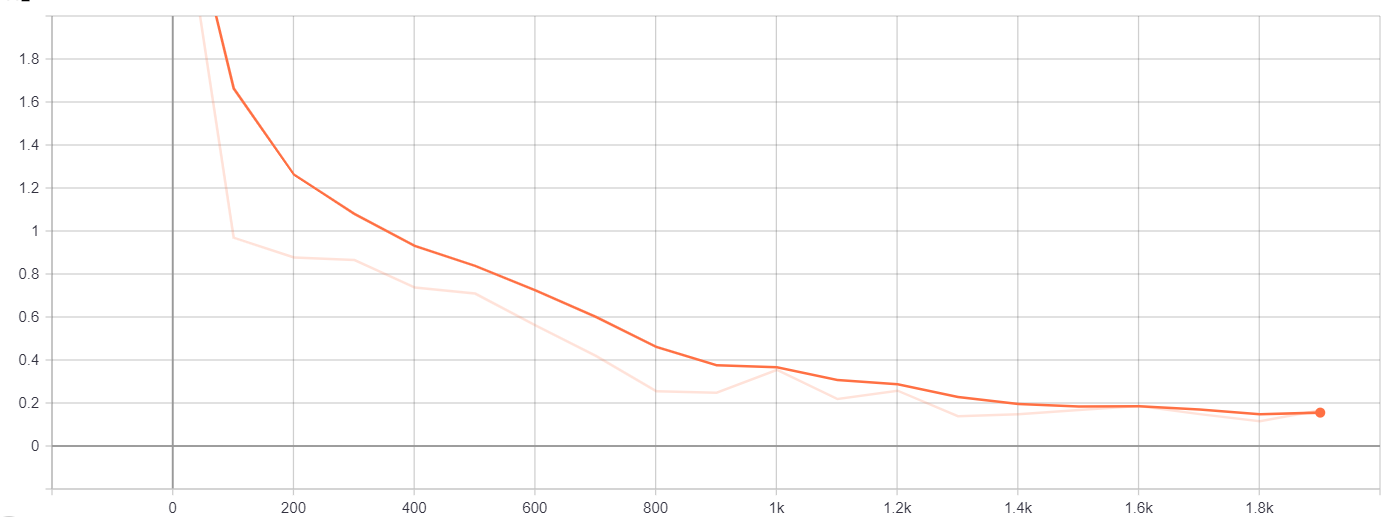
\includegraphics[width=6.27in,height=2.33in]{./media/image1.png}
	\end{Center}
\end{figure}


%%%%%%%%%%%%%%%%%%%% Figure/Image No: 4 Ends here %%%%%%%%%%%%%%%%%%%%

\par

\begin{FlushRight}
Figure 5.1 (Faster R-CNN Inception V2 2000 steps training loss graph)
\end{FlushRight}\par



%%%%%%%%%%%%%%%%%%%% Figure/Image No: 5 starts here %%%%%%%%%%%%%%%%%%%%

\begin{figure}[H]
	\begin{Center}
		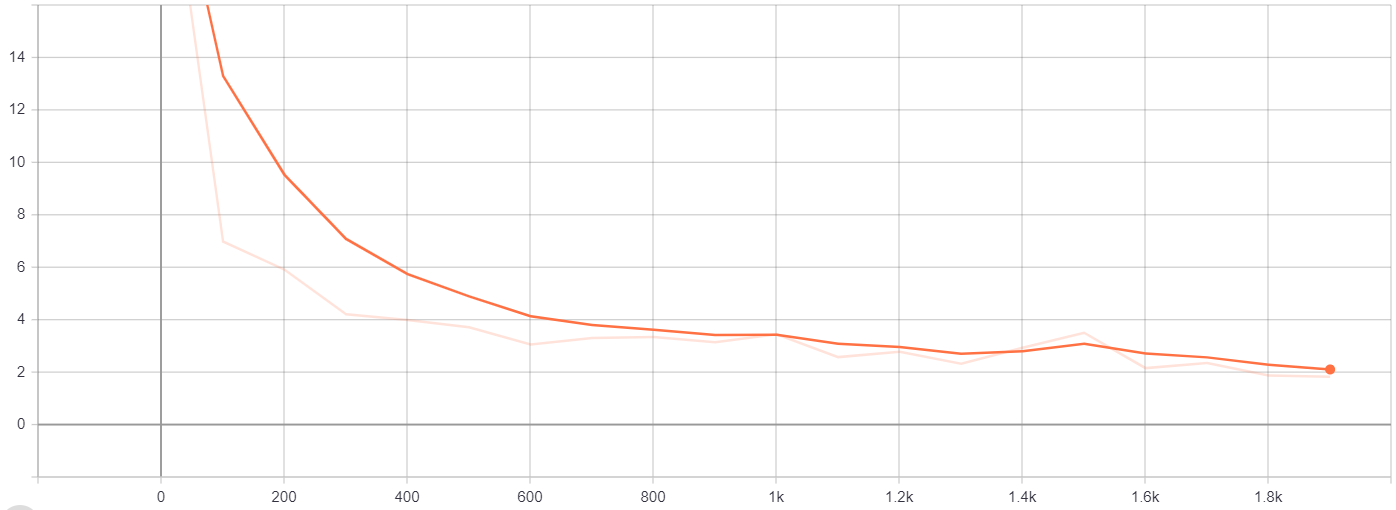
\includegraphics[width=6.27in,height=2.29in]{./media/image9.png}
	\end{Center}
\end{figure}


%%%%%%%%%%%%%%%%%%%% Figure/Image No: 5 Ends here %%%%%%%%%%%%%%%%%%%%

\par

\begin{FlushRight}
Figure 5.2 (SSD Mobilenet V2 2000 steps training loss graph)
\end{FlushRight}\par



%%%%%%%%%%%%%%%%%%%% Figure/Image No: 6 starts here %%%%%%%%%%%%%%%%%%%%

\begin{figure}[H]
	\begin{Center}
		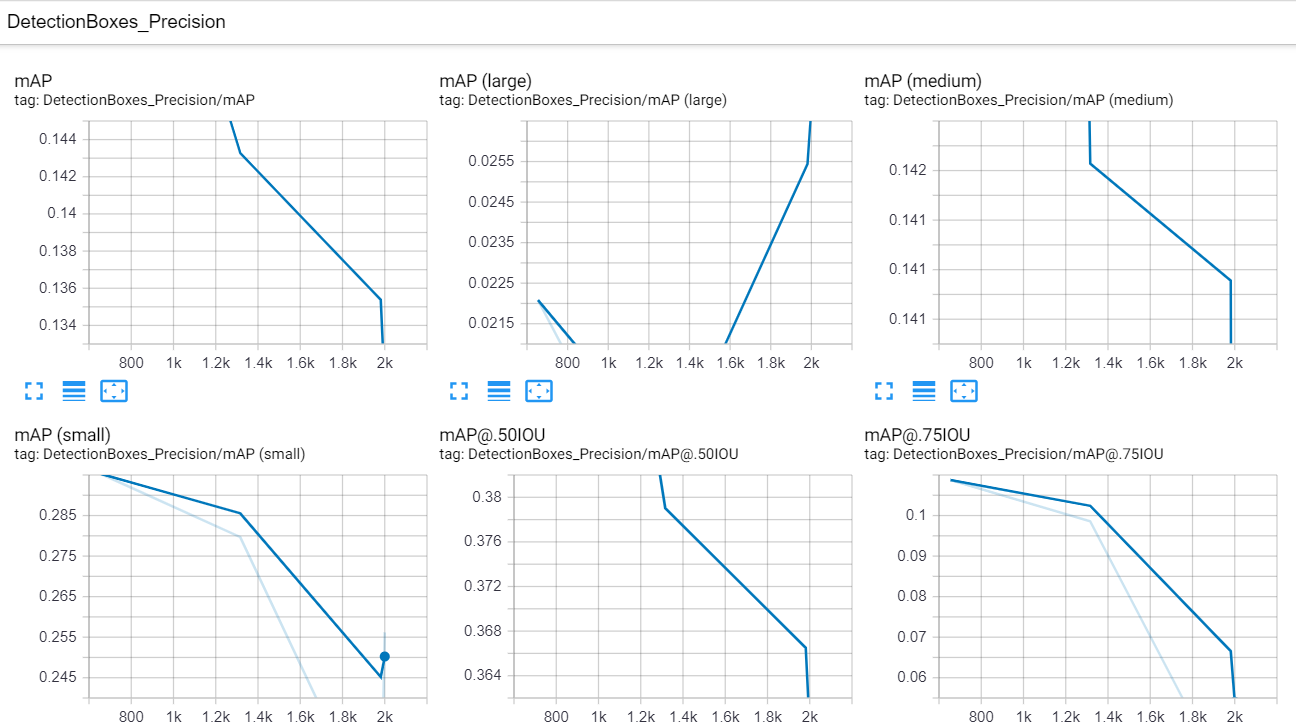
\includegraphics[width=6.27in,height=3.53in]{./media/image3.png}
	\end{Center}
\end{figure}


%%%%%%%%%%%%%%%%%%%% Figure/Image No: 6 Ends here %%%%%%%%%%%%%%%%%%%%

\par

\begin{FlushRight}
Figure 5.3 (Faster R-CNN Inception V2 2000 steps precision/mAP graph)
\end{FlushRight}\par



%%%%%%%%%%%%%%%%%%%% Figure/Image No: 7 starts here %%%%%%%%%%%%%%%%%%%%

\begin{figure}[H]
	\begin{Center}
		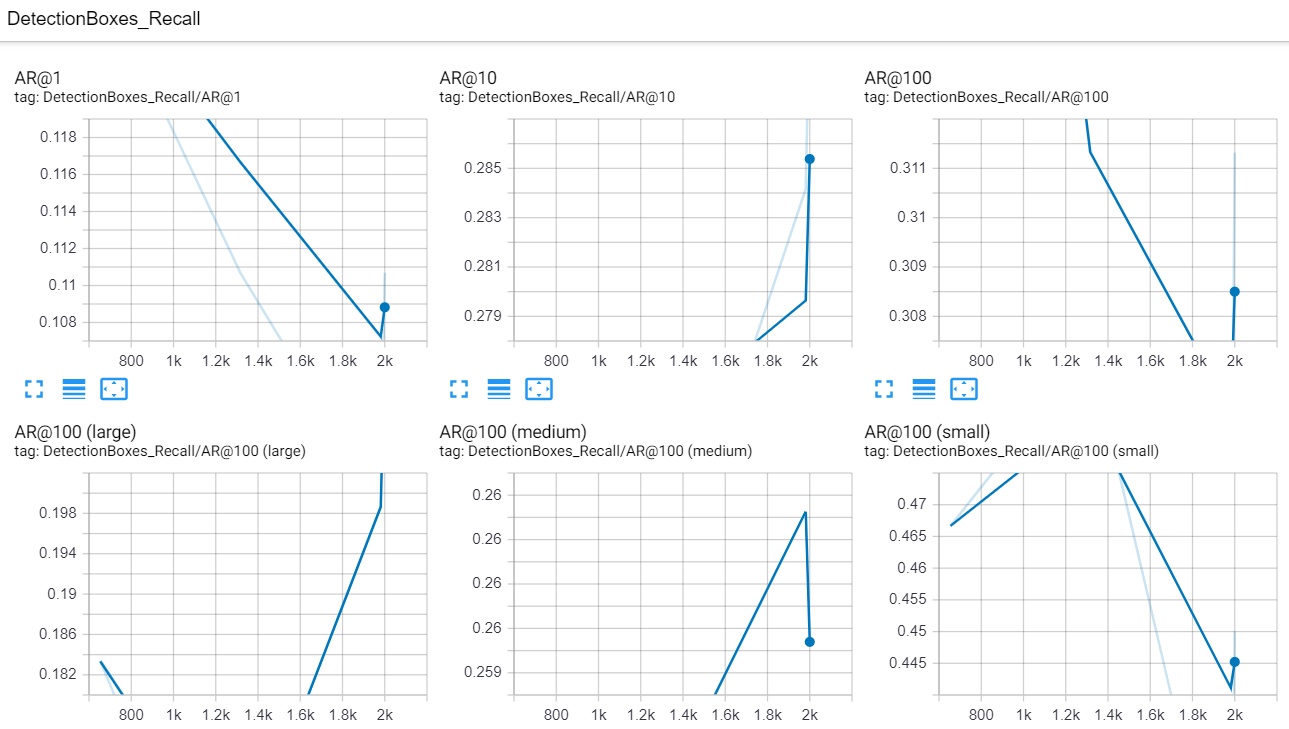
\includegraphics[width=6.27in,height=3.54in]{./media/image2.png}
	\end{Center}
\end{figure}


%%%%%%%%%%%%%%%%%%%% Figure/Image No: 7 Ends here %%%%%%%%%%%%%%%%%%%%

\par

\begin{FlushRight}
Figure 5.4 (Faster R-CNN Inception V2 2000 steps recall graph)
\end{FlushRight}\par


\vspace{\baselineskip}

\vspace{\baselineskip}

\vspace{\baselineskip}

\vspace{\baselineskip}


%%%%%%%%%%%%%%%%%%%% Figure/Image No: 8 starts here %%%%%%%%%%%%%%%%%%%%

\begin{figure}[H]
	\begin{Center}
		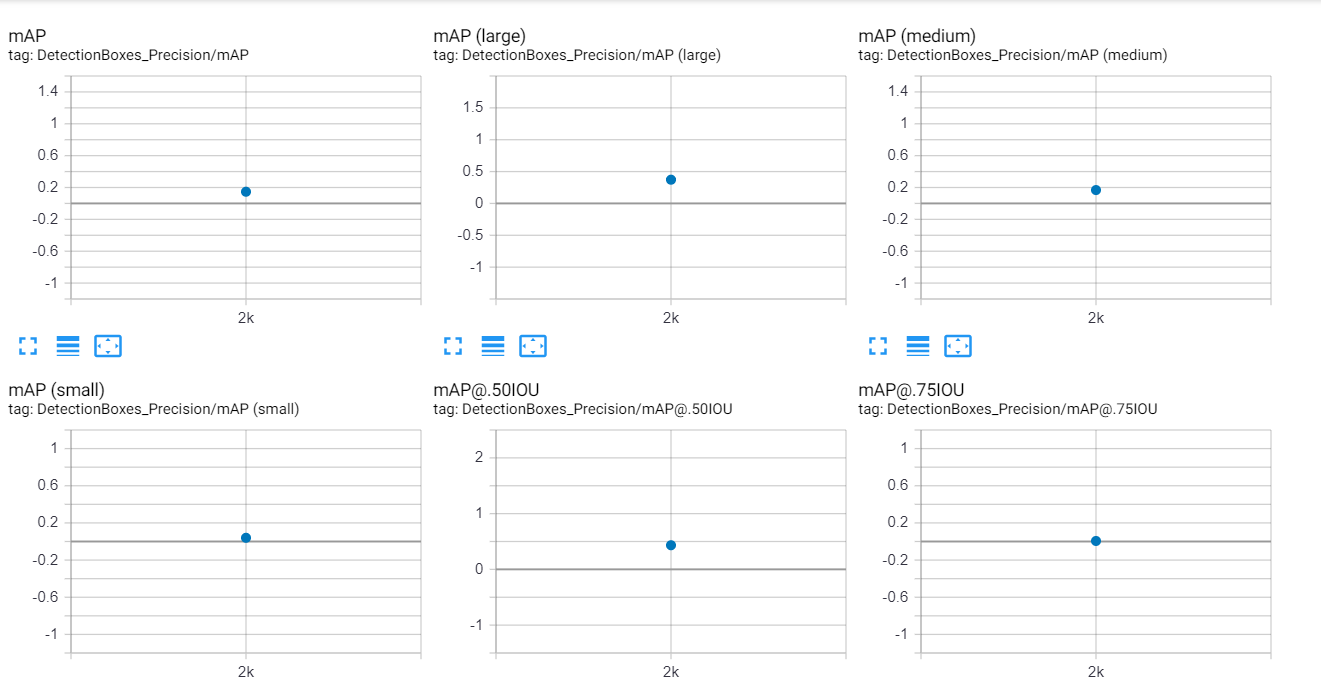
\includegraphics[width=6.27in,height=3.25in]{./media/image11.png}
	\end{Center}
\end{figure}


%%%%%%%%%%%%%%%%%%%% Figure/Image No: 8 Ends here %%%%%%%%%%%%%%%%%%%%

\par

\begin{FlushRight}
Figure 5.5 (SSD Mobilenet V2 2000 steps precision/mAP graph)
\end{FlushRight}\par


\vspace{\baselineskip}


%%%%%%%%%%%%%%%%%%%% Figure/Image No: 9 starts here %%%%%%%%%%%%%%%%%%%%

\begin{figure}[H]
	\begin{Center}
		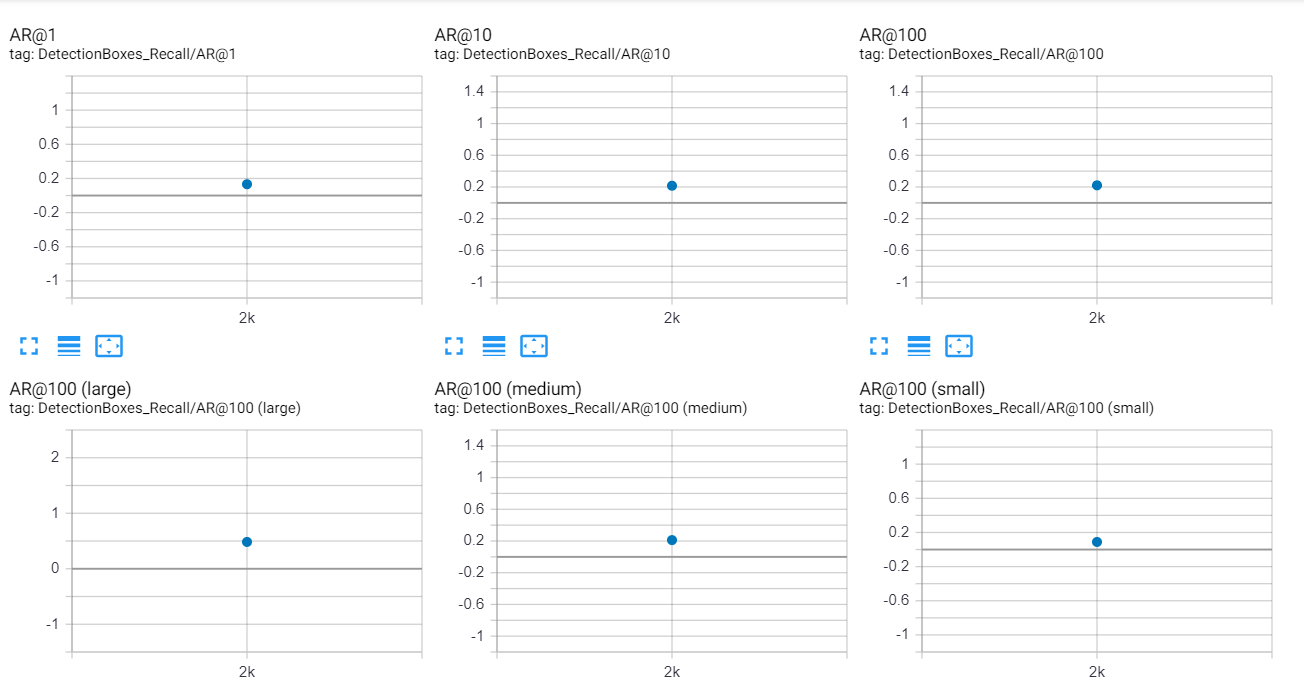
\includegraphics[width=6.27in,height=3.31in]{./media/image8.png}
	\end{Center}
\end{figure}


%%%%%%%%%%%%%%%%%%%% Figure/Image No: 9 Ends here %%%%%%%%%%%%%%%%%%%%

\par

\begin{FlushRight}
Figure 5.6 (SSD MobilNet V2 2000 steps recall graph)
\end{FlushRight}\par


\vspace{\baselineskip}


%%%%%%%%%%%%%%%%%%%% Figure/Image No: 10 starts here %%%%%%%%%%%%%%%%%%%%

\begin{figure}[H]
	\begin{Center}
		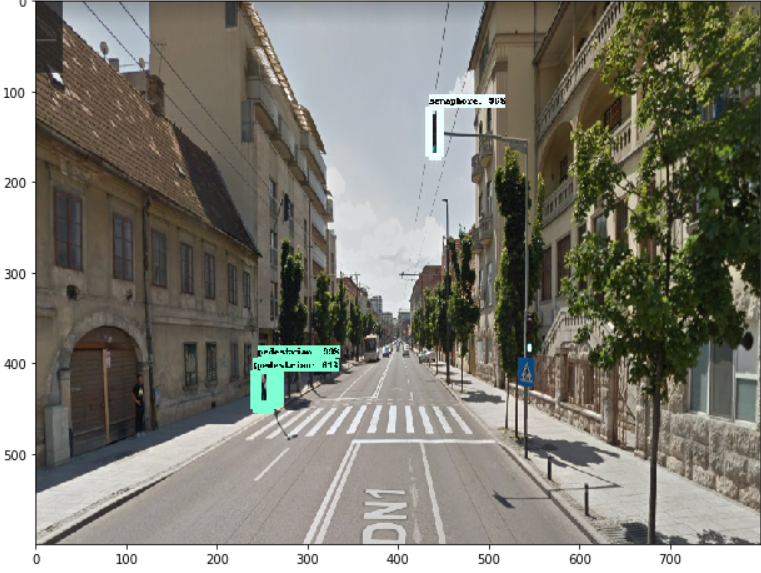
\includegraphics[width=5.01in,height=3.8in]{./media/image5.png}
	\end{Center}
\end{figure}


%%%%%%%%%%%%%%%%%%%% Figure/Image No: 10 Ends here %%%%%%%%%%%%%%%%%%%%

\par

\begin{Center}
Figure 5.7 Faster R-CNN test image 1
\end{Center}\par


\vspace{\baselineskip}


%%%%%%%%%%%%%%%%%%%% Figure/Image No: 11 starts here %%%%%%%%%%%%%%%%%%%%

\begin{figure}[H]
	\begin{Center}
		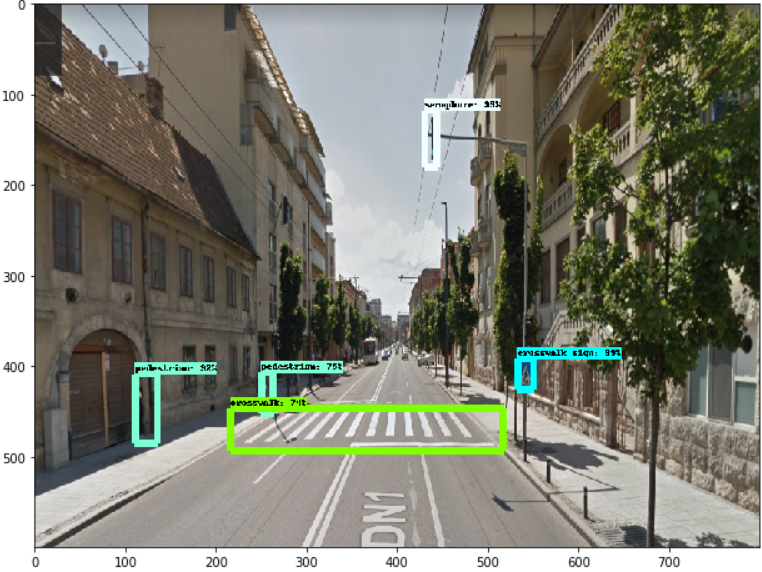
\includegraphics[width=4.98in,height=3.74in]{./media/image7.png}
	\end{Center}
\end{figure}


%%%%%%%%%%%%%%%%%%%% Figure/Image No: 11 Ends here %%%%%%%%%%%%%%%%%%%%

\par

\begin{Center}
Figure 5.8 SSD MobileNet test image 1
\end{Center}\par


\vspace{\baselineskip}
\section{Discussion}
The graphs displayed in the previous subchapter, where 2 pre-trained models (SSD Mobilenet and Faster R-CNN) were used for transfer learning, depict the average precision, average recall and loss function. Taking into account these data, the Faster R-CNN has an average precision of 13,4$\%$  (Figure 5.3) while the SSD Mobilenet has a slightly higher average of around 14$\%$  (Figure 5.5). These values are very low compared to the precision of the pre-trained model of 90$\%$  for Faster R-CNN and 61$\%$  for SSD Mobilenet mainly because of the very small number of training steps. In order to achieve comparable results to the results of the pre-trained models the number of training steps must be increased.\par


\vspace{\baselineskip}
There\ have been made benchmarks on pre-trained models and one of them shows that Faster R-CNN Inception V2 obtains a higher mAP than the SSD Mobilenet, the latter one is the fastest and lightest model in terms of memory consumption, making it an optimal choice for deployment in mobile and embedded devices, however Faster R-CNN Inception V2 is also the lightest model between the R-CNN architecture.[8]  \par


\vspace{\baselineskip}


%%%%%%%%%%%%%%%%%%%% Table No: 1 starts here %%%%%%%%%%%%%%%%%%%%


\begin{table}[H]
 			\centering
\begin{tabular}{p{1.26in}p{1.16in}p{1.14in}p{1.07in}p{0.56in}}
%row no:1
\multicolumn{1}{p{1.26in}}{\Centering \textcolor[HTML]{24292E}{model}} & 
\multicolumn{1}{p{1.16in}}{\Centering \textcolor[HTML]{24292E}{MB}} & 
\multicolumn{1}{p{1.14in}}{\Centering \textcolor[HTML]{24292E}{Total exec (ms)}} & 
\multicolumn{1}{p{1.07in}}{\Centering \textcolor[HTML]{24292E}{CPU(ms)}} & 
\multicolumn{1}{p{0.56in}}{\Centering \textcolor[HTML]{24292E}{mAP}} \\
\hhline{~~~~~}
%row no:2
\multicolumn{1}{p{1.26in}}{\textit{\textcolor[HTML]{24292E}{Faster R-CNN Resnet 50}}} & 
\multicolumn{1}{p{1.16in}}{\textit{\textcolor[HTML]{24292E}{5256.454615}}} & 
\multicolumn{1}{p{1.14in}}{\textit{\textcolor[HTML]{24292E}{104.0363553}}} & 
\multicolumn{1}{p{1.07in}}{\textit{\textcolor[HTML]{24292E}{28.10240132}}} & 
\multicolumn{1}{p{0.56in}}{\textit{\textcolor[HTML]{24292E}{91.52}}} \\
\hhline{~~~~~}
%row no:3
\multicolumn{1}{p{1.26in}}{\textit{\textcolor[HTML]{24292E}{Faster R-CNN Resnet 101}}} & 
\multicolumn{1}{p{1.16in}}{\textit{\textcolor[HTML]{24292E}{6134.705805}}} & 
\multicolumn{1}{p{1.14in}}{\textit{\textcolor[HTML]{24292E}{123.2729175}}} & 
\multicolumn{1}{p{1.07in}}{\textit{\textcolor[HTML]{24292E}{32.9357732}}} & 
\multicolumn{1}{p{0.56in}}{\textit{\textcolor[HTML]{24292E}{95.08}}} \\
\hhline{~~~~~}
%row no:4
\multicolumn{1}{p{1.26in}}{\textcolor[HTML]{24292E}{Faster R-CNN Inception V2}} & 
\multicolumn{1}{p{1.16in}}{\textcolor[HTML]{24292E}{2175.206857}} & 
\multicolumn{1}{p{1.14in}}{\textcolor[HTML]{24292E}{58.53338971}} & 
\multicolumn{1}{p{1.07in}}{\textcolor[HTML]{24292E}{19.76525}} & 
\multicolumn{1}{p{0.56in}}{\textcolor[HTML]{24292E}{90.62}} \\
\hhline{~~~~~}
%row no:5
\multicolumn{1}{p{1.26in}}{\textit{\textcolor[HTML]{24292E}{Faster R-CNN Inception Resnet V2}}} & 
\multicolumn{1}{p{1.16in}}{\textit{\textcolor[HTML]{24292E}{18250.446008}}} & 
\multicolumn{1}{p{1.14in}}{\textit{\textcolor[HTML]{24292E}{442.2206796}}} & 
\multicolumn{1}{p{1.07in}}{\textit{\textcolor[HTML]{24292E}{76062}}} & 
\multicolumn{1}{p{0.56in}}{\textit{\textcolor[HTML]{24292E}{95.77}}} \\
\hhline{~~~~~}
%row no:6
\multicolumn{1}{p{1.26in}}{\textit{\textcolor[HTML]{24292E}{R-FCN Resnet 101}}} & 
\multicolumn{1}{p{1.16in}}{\textit{\textcolor[HTML]{24292E}{3509.75153}}} & 
\multicolumn{1}{p{1.14in}}{\textit{\textcolor[HTML]{24292E}{85.45207971}}} & 
\multicolumn{1}{p{1.07in}}{\textit{\textcolor[HTML]{24292E}{33.04886232}}} & 
\multicolumn{1}{p{0.56in}}{\textit{\textcolor[HTML]{24292E}{95.15}}} \\
\hhline{~~~~~}
%row no:7
\multicolumn{1}{p{1.26in}}{\textcolor[HTML]{24292E}{SSD Mobilenet}} & 
\multicolumn{1}{p{1.16in}}{\textcolor[HTML]{24292E}{94.696119}} & 
\multicolumn{1}{p{1.14in}}{\textcolor[HTML]{24292E}{15.14525}} & 
\multicolumn{1}{p{1.07in}}{\textcolor[HTML]{24292E}{11.12398214}} & 
\multicolumn{1}{p{0.56in}}{\textcolor[HTML]{24292E}{61.64}} \\
\hhline{~~~~~}
%row no:8
\multicolumn{1}{p{1.26in}}{\textit{\textcolor[HTML]{24292E}{SSD Inception V2}}} & 
\multicolumn{1}{p{1.16in}}{\textit{\textcolor[HTML]{24292E}{284.512918}}} & 
\multicolumn{1}{p{1.14in}}{\textit{\textcolor[HTML]{24292E}{23.74428378}}} & 
\multicolumn{1}{p{1.07in}}{\textit{\textcolor[HTML]{24292E}{14.35087838}}} & 
\multicolumn{1}{p{0.56in}}{\textit{\textcolor[HTML]{24292E}{66.10}}} \\
\hhline{~~~~~}

\end{tabular}
 \end{table}


%%%%%%%%%%%%%%%%%%%% Table No: 1 ends here %%%%%%%%%%%%%%%%%%%%


\vspace{\baselineskip}
During the re-trainings of the pre-trained models SSD Mobilenet V2 and Faster R-CNN Inception V2 there’s been a major difference between them, SSD is trained 3 times faster than the Faster R-CNN making it easier for developers to re-train the model faster and tweek the input parameters in order to achieve the best results in terms of accuracy.\par

\chapter{Conclusion and future work}
In conclusion, a mobile application using Artificial Intelligence can reduce the risk of potential danger events in traffic by informing the driver ahead of time. A mobile application is easy to use and can easily be used in any vehicle.\par

Moreover, as time passes by, AI algorithms and models increase their efficiency, making these kind of applications more trustful and efficient.\par

A possible future improvement is to add more traffic signs to the model in order for the system to identify all possible route dangers.\par

Taking into account the fact that more traffic signs can be recognized, an algorithm can be implemented, in order to send more accurate danger signals taking into consideration more factors, such as weather conditions, driver’s current state of mind, car’s real-time statistics (speed, car defects, and so on).\par

\par

\chapter{References}

\begin{justify}
[1] The TensorFlow Authors (2019) TensorFlow Object Detection API (readme). URI: \href{https://github.com/TensorFlow/models/tree/master/research/object_detection}{\textcolor[HTML]{1155CC}{\ul{https://github.com/TensorFlow/models/tree/master/research/object\_detection}}}.
\end{justify}\par


\vspace{\baselineskip}
\begin{justify}
[2] Common Object in Context (2019) documentation. URI: \href{http://cocodataset.org/#home}{\textcolor[HTML]{1155CC}{\ul{http://cocodataset.org/$\#$ home}}}
\end{justify}\par


\vspace{\baselineskip}
\begin{justify}
[3] Review: MobileNetV2 — Light Weight Model (Image Classification), Sik-Ho Tsang, May 19, 2019, 
\end{justify}\par

\begin{justify}
URI:\href{https://towardsdatascience.com/review-mobilenetv2-light-weight-model-image-classification-8febb490e61c}{\textcolor[HTML]{1155CC}{\ul{https://towardsdatascience.com/review-mobilenetv2-light-weight-model-image-classification-8febb490e61c}}}
\end{justify}\par


\vspace{\baselineskip}
\begin{justify}
[4]\ MobileNetV2: Inverted Residuals and Linear Bottlenecks,  Paul-Louise Pröve, URI: \\
\href{https://towardsdatascience.com/mobilenetv2-inverted-residuals-and-linear-bottlenecks-8a4362f4ffd5}{\textcolor[HTML]{1155CC}{\ul{https://towardsdatascience.com/mobilenetv2-inverted-residuals-and-linear-bottlenecks-8a4362f4ffd5}}}
\end{justify}\par


\vspace{\baselineskip}
\begin{justify}
[5] Faster RCNN Object detection, Achraf KHAZRI, Apr 9, 2019, URI:
\end{justify}\par

\begin{justify}
 \href{https://towardsdatascience.com/faster-rcnn-object-detection-f865e5ed7fc4}{\textcolor[HTML]{1155CC}{\ul{https://towardsdatascience.com/faster-rcnn-object-detection-f865e5ed7fc4}}}
\end{justify}\par


\vspace{\baselineskip}
\begin{justify}
[6] ImageNet (2019) Documentation, URI: \href{http://www.image-net.org/}{\textcolor[HTML]{1155CC}{\ul{http://www.image-net.org/}}}
\end{justify}\par


\vspace{\baselineskip}
\begin{justify}
[7] LabelImg (readme). URI: \href{https://github.com/tzutalin/labelImg}{\textcolor[HTML]{1155CC}{\ul{https://github.com/tzutalin/labelImg}}}
\end{justify}\par


\vspace{\baselineskip}
\begin{justify}
[8] Traffic Sign Detection, \href{https://github.com/aarcosg/traffic-sign-detection}{\textcolor[HTML]{1155CC}{\ul{https://github.com/aarcosg/traffic-sign-detection}}}
\end{justify}\par


\vspace{\baselineskip}
\begin{justify}
[9]\ AccuWeather,  \href{https://en.wikipedia.org/wiki/AccuWeather}{\textcolor[HTML]{1155CC}{\ul{https://en.wikipedia.org/wiki/AccuWeather}}}
\end{justify}\par

[10] BMW Intelligent Driving, \href{https://www.bmw.ca/en/topics/experience/connected-drive/bmw-connecteddrive-driver-assistance.html}{\textcolor[HTML]{1155CC}{\ul{https://www.bmw.ca/en/topics/experience/connected-drive/bmw-connecteddrive-driver-assistance.html}}}\par


\printbibliography
\end{document}